\subsection*{Task 5.4}

The response of a PID-controller is calculated as:

\begin{align*}
	\tau(t) &= k_p \cdot e(t) + k_v \cdot \dot{e}(t) + k_i \int_{t_o}^{t}e(t')dt'
\end{align*}

We consider the error $e(t)$ to be $0$ at the beginning ($t_0$).
Therefore, $e(t), \dot{e}(t)$ and $\int_{t_o}^{t}e(t')dt'$ are $0$ for $t < 0$.

\subsubsection*{5.4.1}

For the heavy-side function as target function the derivative is the Dirac delta function, which is infinite at $t=0$
\begin{align*}
	\delta(t) &= 
	\begin{cases}
		\infty, & t = 0\\
		0, & t \ne 0 
	\end{cases}
\end{align*}
Theoretically the PID-controller is able to set the correct response of infinite at $t=0$ and the error will be $0$ again afterwards.
Overall, the response is then:

\begin{align*}
\tau(t) &= 
\begin{cases}
0, & t < 0\\
\infty, & t = 0\\
0, & t > 0
\end{cases}
\end{align*}

In real applications the correct value won't be reached instantaneous at $t=0$, so that the response will form a flattening curve.\medskip

If the input value is not changed over time and stays at $0$, the target function and the error function are equal: $y(t) = e(t)$.
In that case $e(t) = 1, \dot{e}(t) = 0$ and $\int_{t_o}^{t}e(t')dt' = \int_{t_o}^{t} 1 dt' = t$ for $t > 0$.
The response of the PID-controller is then:
\begin{align*}
\tau(t) &= 
\begin{cases}
0, & t < 0\\
\infty, & t = 0\\
k_p + k_i \cdot t, & t > 0 
\end{cases}
\end{align*}

\begin{figure}[!h]
\centering
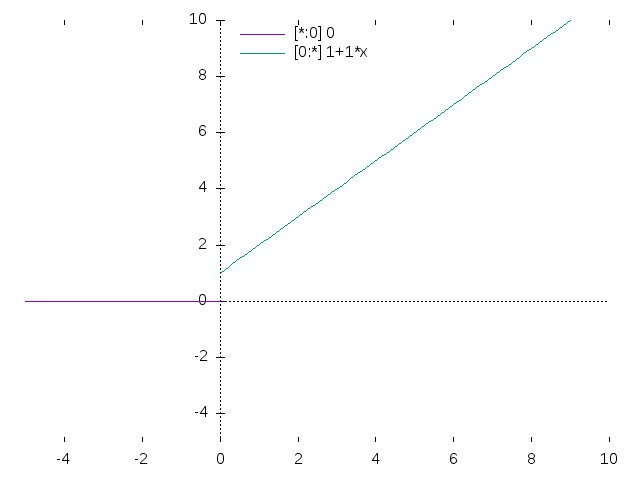
\includegraphics[width= 0.65\textwidth ]{task541.png}
\caption{Output of the PID-controller on the heavy-side function.}
\end{figure}

\subsubsection*{5.4.2}

Considering again that error and target function are equal.\\
The derivative of the error function (ramp function) is the heavy-side function.
And $e(t) = t$ and $\int_{t_o}^{t}e(t')dt' = \int_{t_o}^{t}t'dt' = \frac{1}{2}t^2$ for $t > 0$.\\
The response of the PID-controller is then:
\begin{align*}
\tau(t) &= 
\begin{cases}
0, & t < 0\\
k_p \cdot t + k_v + k_i \cdot \frac{1}{2}t^2, & t \ge 0
\end{cases}
\end{align*}

\begin{figure}[!h]
	\centering
	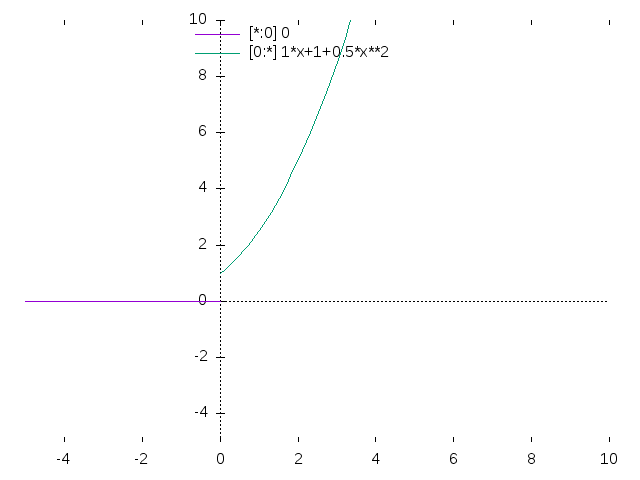
\includegraphics[width= 0.65\textwidth ]{task542.png}
	\caption{Output of the PID-controller on the ramp function.}
\end{figure}




